%
\providecommand{\main}{../..}
\documentclass[../../main.tex]{subfiles}

\begin{document}

\lesson{15}{15/4/20}

%Add derivation of S_I (interpretation as function of ignorance), CFR ex. 5.17
%Verify the three properties on the final function

\section{Information Entropy and Ignorance}
The definition we gave of \textbf{information entropy} in the last section, as the average \q{surprise} of data sampled from a distribution, may seem quite arbitrary and contrived.

\medskip

A much more \textit{natural} way to derive (\ref{eqn:S-info-discrete}) is to interpet it as a measure of the amount of \textbf{ignorance} or \textbf{uncertainty} contained in a probability distribution. In other words, if $S_I[\rho]$ is maximum, then $\rho$ possess the \textit{least amount of} \textbf{bias}.  

\medskip

Recall that previously we assumed $S_I[\rho]$ to be the average information \textit{gain} that can be obtained from data distributed according to $\rho$. Intuitively, we \textit{discover more} when $\rho$ is \q{uncertain}, i.e. when it is difficult to even approximately predict new observations before they are made. Conversely, if $\rho$ is \textit{peaked} around some value $x$, and we observe $x$ in an experiment, we gain almost no \q{new} information, as we have obtained an \textit{unsurprising} result. So, in a sense, we can \q{learn the most when we initially know the least}. 

\medskip

While it is not easy to exactly define what we mean by \q{ignorance}, we can still find some key properties any \textit{ignorance}-measure should have, and use them to fix the functional form of $S_I$.

\medskip

So, let's suppose $S_I(\bm{p})$ to be a measure of the \textit{uncertainty} of the discrete distribution $\bm{p} = (p_1, \dots, p_\Omega)$, with $\sum_{i=1}^{\Omega} p_i = 1$. We require the following $3$ properties:
\begin{enumerate}
    \item \textbf{Uniform distribution = maximum ignorance},\marginpar{The $3$ properties of ignorance} i.e.:
    \begin{align} \label{eqn:key1}
        \displaystyle S_I \left(\frac{1}{\Omega}, \dots, \frac{1}{\Omega}  \right) > S_I (p_1, \dots, p_{\Omega})
    \end{align}
     for all $\bm{p}$ that are non-uniform (i.e. such that not all $p_i$ are the same).  

    \medskip

    Clearly, if not all $p_i$ are the same, then some states are more probable than others, meaning that we possess some bias towards them. The uncertainty is maximum for a uniform distribution, as in that case we have no bias towards any state at all.

    \item \textbf{Impossible events do not alter the uncertainty}:
    \begin{align*}
        S_I(p_1, \dots, p_{\Omega},0) = S_I(p_1, \dots, p_{\Omega})
    \end{align*} 
    If a state is never visited, then it makes no difference on the amount of knowledge we possess about the distribution. This makes $S_I$ \textit{consistent}, since we can always extend the domain of a distribution $\bm{p}$ by adding $0$\textit{s}, and this should not change any property of $\bm{p}$.

    \item \textbf{Rule for updating knowledge}. If two random variables $A$ and $B$ are not independent, then observing one of them tells us something about the other. Let's define $S_I(A)$ as the amount of uncertainty contained in the distribution $\bm{p}$ of $A$, and similarly $S_I(B)$ for the distribution $\bm{q}$ of $B$. If we consider both of them at the same time, their \textit{total uncertainty} will be the one of their joint distribution $S_I(AB)$.
    
    Suppose that we measure $B$, and find it equal to a certain state $B_l$. Since one of the two variables is now fixed, we know something more about $AB$. In particular, $A$ must be \textit{compatible} with the observation of $B_l$. So, our final ignorance is given by $S_I(A|B_l)$, where $A|B_l$ is the \textit{conditional distribution} of $A$ given the fact that we observed $B_l$.

    It is then natural to require that, \textit{on average}, the reduction in ignorance from $S_I(AB)$ to $S_I(A|B_l)$ is given exactly by the amount of ignorance $S_I(B)$ contained in $B$:
    \begin{align*}
        S_I(AB) - \langle S_I(A|B_l) \rangle = S_I(B)
    \end{align*}
    In other words, recall that $S_I(B)$ is the \textit{average} gain of information by observing $B$, which reduces our ignorance from $S_I(AB)$ to $\langle S_I(A|B_l)\rangle$.
\end{enumerate}

We will now show that there exists\marginpar{Proof for the form of Shannon's entropy} a unique \textbf{continuous} function $S_I$ (up to a multiplicative constant) satisfying all of these $3$ properties.

\medskip

Let $\bm{p} = (p_1,\dots,p_\Omega)$ be the distribution of $A$, and $\bm{q} = (q_1,\dots, q_{M})$ that of $B$. Then:
\begin{align*}
    S_I(A) &\equiv S_I(\bm{p}) = S_I(p_1, \dots, p_\Omega)\\
    S_I(B) &\equiv S_I(\bm{q}) = S_I(q_1, \dots, q_M)
\end{align*}
Their joint distribution is denoted as:
\begin{align*}
    \mathbb{P}[A=i, B=j] = \underbrace{\mathbb{P}[A=i|B=j]}_{c_{ij}}  \underbrace{\mathbb{P}[B=j]}_{q_j} = c_{ij} q_j \quad \substack{1 \leq i \leq \Omega\\1 \leq j \leq M}
\end{align*}
And so:
\begin{align*}
    \langle S_I(A|B_l) \rangle_B &\equiv \sum_{l=1}^M q_l S_I(c_{1l}, \dots, c_{\Omega l})\\
    S_I(AB) &\equiv S_I(c_{11} q_1, \dots, c_{\Omega M} q_M)
\end{align*}

Having established the notation, we start by rewriting $S_I(B)$ in terms of the entropy of a \textit{uniform} distribution $L(g)$ defined as follows:
\begin{align*}
    L(g) \equiv S_{I}\left(\frac{1}{g},\dots,\frac{1}{g}\right)
\end{align*}
The idea is that $L(g)$ will be easier to determine, since it depends only on one argument $g$. To do this, we use property $3$:
\begin{align}\label{eqn:prop3-b}
    S_I(B) = S_I(AB) - \langle S_I(A|B_l) \rangle_B
\end{align}
If we choose $A$ with a distribution $\bm{p}$ such that $AB$ has a uniform distribution $p_{ij} = 1/g$, then $S_I(AB) = L(g)$. So:
\begin{align*}
    \mathbb{P}[A=k, B=l] \overset{!}{=} \frac{1}{g} = \mathbb{P}[A=k|B=l] \mathbb{P}[B=l] = c_{kl} q_l 
\end{align*}
Suppose for simplicity that all $q_l \in \mathbb{Q}$, and can be written as $q_l = g_l/g$, where $g_l, g \in \mathbb{N}$ and $g$ is their least common denominator. In this way:
\begin{align*}
    \frac{1}{\cancel{g}} \overset{!}{=}  c_{kl} \frac{g_l}{\cancel{g}} \Rightarrow \mathbb{P}[A=k|B=l] = c_{kl} = \frac{1}{g_l} 
\end{align*}
and so also the conditional distribution is uniform, meaning that:
\begin{align*}
    \langle S_I(A|B_l) \rangle_B = \sum_{l=1}^M q_l S_I(c_{1l},\dots, c_{\Omega l}) = \sum_l q_l S_I\left(\frac{1}{g_l},\dots,\frac{1}{g_l}  \right) = \sum_l q_l L(g_l)
\end{align*}
Substituting back in (\ref{eqn:prop3-b}) we get:
\begin{align*}
    S_I(B) = L(g) - \sum_l q_l L(g_l) \qquad q_l \in \mathbb{Q}
\end{align*}
which can be uniquely extended to $q_l \in \mathbb{R}$ by \textbf{continuity}, since the set of rational numbers is \textit{dense} in $\mathbb{R}$.

\medskip

So, all that's left is to find an expression for the entropy $L(g)$ of a uniform distribution. First, note that if we can prove that $L(g) = k_B \log g$, then $S_I$ is exactly Shannon's entropy:
\begin{align*}
    S_I(B) &= k_B \log g - \sum_{l=1}^M q_l k_B \log g_l = k_B \underbrace{\textcolor{Red}{\sum_{l=1}^M q_l}}_{1}  \log g - \sum_{l=1}^M q_l k_B \log g_l =\\
    &= -k_B \sum_{l=1}^M \Big( q_l \log g_l - q_l \log g \Big) = -k_B \sum_{l=1}^M q_l \log \underbrace{\frac{g_l}{g}}_{q_l} = \\
    &= -k_B \sum_{l=1}^M q_l \log q_l \qquad q_l \in \mathbb{Q}  
\end{align*}
which can then be uniquely extended by continuity to $q_l \in \mathbb{R}$.

\medskip

So, we need to prove that, up to a multiplicative constant, $L(g)$ is a logarithm. We start by first showing that it satisfies the defining properties of a logarithm:

\begin{itemize}
    \item $L(g)$ is \textit{monotone increasing} with $g$. In fact:
    \begin{align*}
        L(g+1) &= S_{I} \left(\frac{1}{g+1},\dots, \frac{1}{g+1}  \right) \underset{(1)}{>} S_I\left(\frac{1}{g}, \dots, \frac{1}{g}, 0\right) =\\
        &\underset{(2)}{=} S_I\left(\frac{1}{g},\dots,\frac{1}{g} \right) \equiv L(g) \qquad \forall g
    \end{align*}
    Due to the first requirement, any non-uniform distribution has a strictly lower entropy than the uniform distribution. In particular, this holds for the distribution that \textit{excludes} the last state. But then we can use the second requirement to \textit{restrict} the domain, since states that are never visited do not impact the entropy.
    \item $L(g^n) = n L(g)$. Let's start with $n=2$. The idea is that $1/g^2$ is the joint distribution of two \textit{uniform} and \textit{independent} random variables with $g$ possible states. Consider the third requirement:
    \begin{align*}
        S_I(AB) = S_I(B) + \langle S_I(A|B_l) \rangle_B
    \end{align*}
    If $A$ and $B$ are independent, then $\langle S_I(A|B_l) \rangle_B = S_I(A)$, since measuring $B$ does not give any information about $A$. Then, if $A$ and $B$ are both uniform over $g \in \mathbb{N}$ states, we have $S_I(B) = S_I(A) = L(g)$. So:
    \begin{align*}
        L(g^2) = S_I(AB) = S_I(A) + S_I(B) = 2 L(g)
    \end{align*}
    The case for generic $n$ can be then proved by induction. If $L(g^n) = n L(g)$ holds for $n$, for $n+1$ we have:
    \begin{align*}
        L(g^{n+1}) = L(g^n) + L(g) = n L(g) + L(g) = (n+1) L(g)
    \end{align*}
    And so $L(g^n) = nL(g) \> \forall n \in \mathbb{N}$.
\end{itemize}
We are now ready to show that $L(g)$ must have the form of a logarithm. Note that, if $2^m < s^n < 2^{m+1}$, then:
\begin{align*}
    2^m < s^n < 2^{m+1} \underset{(a)}{\Rightarrow}  \log (2^m) < \log(s^n) < \log(2^{m+1}) \underset{(b)}{\Rightarrow}  m \log 2 < n \log s + (m+1)\log 2
\end{align*}
and dividing by $n \log 2$ leads to:
\begin{align}\label{eqn:ineq1}
    \frac{m}{n} < \frac{\log s}{\log 2} < \frac{m+1}{n}   
\end{align}
In (a) we have used the fact that $\log x$ is monotonic increasing, and in (b) the fact that $\log(a^n) = n \log a$. But the same two properties hold also for $L(g)$, and so we have:
\begin{align}\label{eqn:ineq2}
    \frac{m}{n} < \frac{L(s)}{L(2)} < \frac{m+1}{n}   
\end{align}
Then, subtracting (\ref{eqn:ineq2}) from (\ref{eqn:ineq1}) we get:
\begin{align*}
    \frac{m}{n} - \frac{m+1}{n} < \frac{L(s)}{L(2)} - \frac{\log s}{\log 2} < \frac{m+1}{m} - \frac{m}{n} \span \\
    \span \Rightarrow -\frac{1}{n} < \frac{L(s)}{L(2)} - \frac{\log s}{\log 2} < \frac{1}{n} \Rightarrow \left | \frac{L(s)}{L(2)} - \frac{\log s}{\log 2}   \right | < \frac{1}{n}  \xrightarrow[n \to +\infty]{} 0 
\end{align*}
which proves that:
\begin{align*}
    L(s) = \underbrace{\frac{L(2)}{\log 2}}_{k} \log s = k \log s  
\end{align*}
for some multiplicative constant $k$.
\begin{flushright}
    $\square$
\end{flushright}

To check that all the previous steps were right, we can verify that $S_I(\bm{p}) = -k_B \sum_i p_i \log p_i$ indeed satisfies all the required properties $1-3$.

\begin{enumerate}
    \item \textbf{Entropy is maximum for uniform distributions}:
    \begin{align*}
        S_I\left(\frac{1}{\Omega},\dots, \frac{1}{\Omega}  \right) > S_I(p_1, \dots, p_\Omega) \qquad \forall \bm{p} \text{ s.t. not all $p_i = 1/\Omega$} 
    \end{align*}
    For simplicity, let's fix $k_B = 1$. Then we note that $f(p) = - p \log p$ is a \textit{concave} function:
    \begin{align*}
        f'(p) &= -[\log p + \frac{p}{p} ] = -[\log p + 1]\\
        f''(p) &= - \frac{1}{p} < 0 \qquad \forall p \in (0,1] 
    \end{align*}
    For a concave function, the average value of $f(p)$ computed over a set $\{p_1,\dots,p_\Omega\}$ is not greater than $f$ evaluated at the average $\bar{p}$:
    \begin{align}\label{eqn:Jensen-ineq}
        \frac{1}{\Omega} \sum_{k=1}^\Omega f(p_k) \leq f\left(\frac{1}{\Omega} \sum_{k=1}^\Omega p_k \right) 
    \end{align}
    This is the so-called Jensen's inequality. %A \textit{graphical} proof is shown in fig. \ref{fig:jensen}. %TODO Add the graphical interpretation

    %TODO Complete from there
\end{enumerate}



\section{MaxEnt Principle}
The main \textit{idea} of the \textbf{MaxEnt}\marginpar{Main idea} principle is to find the \textbf{most general} probability distribution \textbf{compatible} with a set of \textbf{constraints} - i.e. \textit{conservation laws} or \textit{measurements} - by \textbf{maximizing} the \textbf{information entropy} $S_I$ subject to these constraints. As $S_I$ can be interpreted as a measure of \textit{ignorance}, the MaxEnt principle merely suggests to choose the most \q{unbiased} distribution, i.e. the one with \q{just enough information} to satisfy the constraints, without containing any further assumption. 

\medskip

In Statistical Mechanics,\marginpar{MaxEnt in Statistical Mechanics} when constructing a macrostate we may \textit{control} only a few macroscopic parameters $\{O_i\}$ - i.e. the energy, the volume, etc. Still, the majority of the system's degrees of freedom are \textit{not} under control: we cannot choose the exact \textit{microstate} the system will be in. At any given moment, the system is \textit{in a single definite microstate} - but we do not know which one. Thus we assign \textit{probabilities} to each microstate, expressing our degree of belief about them\footnote{In the Bayesian sense}, i.e. how much we suspect that a certain microstate may be the \q{real} one. There are many possible choices for these probabilities. For sure, they must be compatible with our previous observations $\{O_i\}$ - and so any microstate which would lead to some different value for the measurements must have a probability $0$. Apart from this, our assignment of probabilities will be arbitrary. However, note that many possible choices of $p_i$, while compatible with the observed $\{O_i\}$ are \textit{biased} towards some measurement values $B_j$ that we do not have under control. MaxEnt tells us to choose $p_i$ such that this \textit{bias} is removed: if we have not measured any $B_j$, then the $p_i$ we choose must weigh each possible value of $B_j$ \textbf{equally}, i.e. \textit{maximize} our ignorance about any other observable which is not under our control. Practically, if we have fixed energy and volume, we know nothing about pressure\footnote{Except in the ideal gas case, but here we are talking in general}, and so we must choose a microstate pdf (i.e. an ensemble) which treats all possible $p$ equally. 

\begin{appr}\textbf{MaxEnt and Bayesian statistics}. MaxEnt is often used as a way to construct \textbf{prior} distributions, encoding all the \q{available} knowledge about some system. Then, in the framework of Bayesian statistics, subsequent observations can be used to \q{update} the prior pdf through Bayes theorem, allowing inference (or learning) from data.  
\end{appr}

\subsection{Single constraint: probability normalization}
Mathematically, to maximize a function ($S_I$) subject to some constraints we use the method of Lagrange multipliers.

\begin{expl}\textbf{Brief refresher of Lagrange multipliers}. Suppose we have two functions $F, g\colon \mathbb{R}^2 \to \mathbb{R}$, with $F(x,y)$ being the function to maximize, and $g(x,y) = c \in \mathbb{R}$ a constraint. 
    
A stationary point $(x_0,y_0)$ of $F$ subject to the constraint $g(x,y) = c$ is such that if we move slightly from $(x_0,y_0)$ along the contour $g(x,y) = c$, the value of $F(x,y)$ does not change (to first order). This happens if the contour of $F$ passing through the stationary point $F(x,y) = F(x_0, y_0)$ is \textbf{tangent} at $(x_0,y_0)$ to that of $g(x,y) = c$ (fig. \ref{fig:contours}), meaning that at $(x_0, y_0)$ the gradients of $F$ and $g$ are parallel:
    \begin{align*}
        \nabla_{x,y} F = \lambda \nabla_{{x,y}} g \qquad \lambda \in \mathbb{R}
    \end{align*}
    (Here we assume that $\nabla_{x,y} g (x_0,y_0) \neq \bm{0}$). Rearranging:
    \begin{align*}
        \nabla_{x,y} (F(x,y) - \lambda g(x,y)) = \bm{0}
    \end{align*}
    Together with the constraint equation $g(x,y) = c$, we have now $3$ equations in $3$ unknowns ($x,y,\lambda$) that can be solve to yield the desired stationary point $(x_0, y_0)$.

    \medskip

    This procedure can be extended to the $n$-dimensional case $F(\bm{x})$, with $d$ constraints $\bm{g}(\bm{x}) = (g_1(\bm{x}), \dots, g_d(\bm{x})) = (c_1,\dots,c_d) = \bm{c}$:
    \begin{align*}
        \grad_{\bm{x}} \left(F(\bm{x}) - \sum_{i=1}^d \lambda_i g_i(\bm{x})\right) = \bm{0}
    \end{align*}
    The parameters $\bm{\lambda} = (\lambda_1, \dots, \lambda_d)$ are called the \textbf{Lagrange multipliers}.  
\end{expl}

\begin{figure}[H]
    \centering
    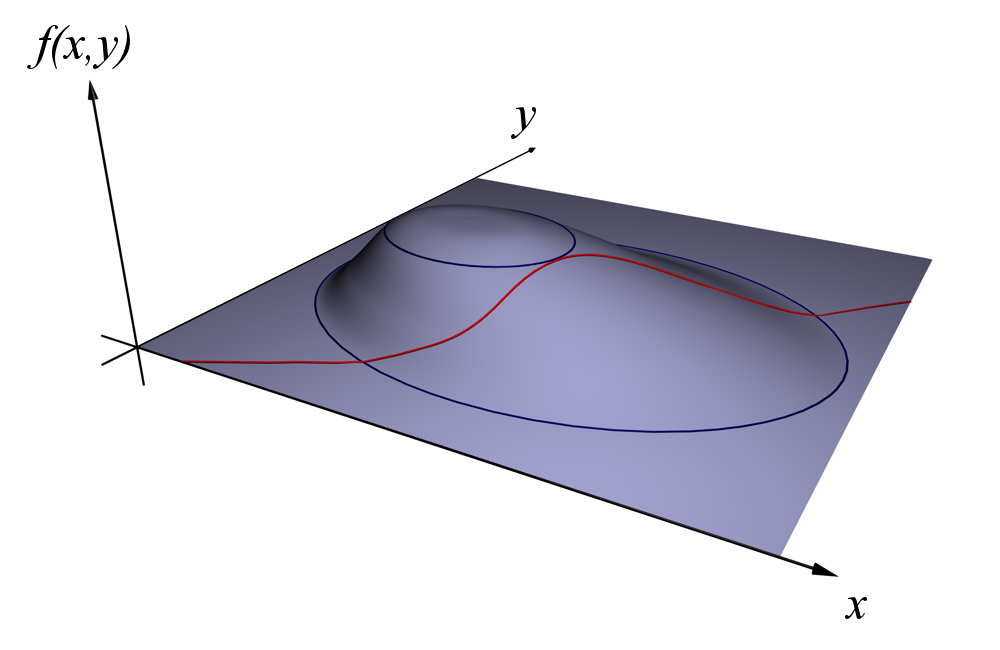
\includegraphics[width=0.6\textwidth]{contours.png}
    \caption{A contour $F(x,y) = F(x_0,y_0)$ is the blue line, while $g(x,y) = c$ is the red line. If we move along the latter near the point where the two lines are tangent, then the value of $F$ will not change (to first order). }
    \label{fig:contours}
\end{figure}


For example, consider\marginpar{First example of MaxEnt} a discrete distribution over a (disjoint) partition of state-space $\Omega$ in $K$ states $\{A_i\}_{i=1,\dots,K}$, with $\mathbb{P}[A_i] = p_i$. Without further knowledge, the only constraint we have on the $\{p_i\}$ is the one given by normalization:
\begin{align*}
    \sum_{i=1}^K p_i \overset{!}{=}  1
\end{align*}
We choose $\{p_i\}$ following the MaxEnt principle:
\begin{align*}
    \max_{\bm{p} \colon \sum_i p_i = 1} S_I(p_1, \dots, p_K)
\end{align*}
which is solved with Lagrange multipliers:
\begin{align*}
    0 &= \pdv{p_j} \left(S_I(\bm{p}) + \lambda \sum_{i=1}^K p_i\right) = -k_B \left[\pdv{p_j} \sum_{i=1}^K p_i \log p_i \right] + \lambda=\\
    &= -k_B \left[\sum_{i=1}^K \delta_{ij} \log p_j + p_i \delta_{ij} \frac{1}{p_j} \right] + \lambda =\\
    &= -k_B(\log p_j + 1) + \lambda = 0 \qquad \forall j=1,\dots,K
\end{align*}
Rearranging:
\begin{align*}
    \ln p_j = \frac{\lambda}{k_B} - 1 \Rightarrow p_j = \exp\left(\frac{\lambda}{k_B} -1 \right)  = \text{constant}  \qquad \forall j=1,\dots,K
\end{align*}
Then by imposing the normalization:
\begin{align*}
    \sum_{i=1}^K p_i = 1 \Leftrightarrow 
    K \exp\left(\frac{\lambda}{k_B} - 1 \right) = 1 \Leftrightarrow \underbrace{\exp\left(\frac{\lambda}{k_B} - 1 \right) }_{p_j} = \frac{1}{K} \Leftrightarrow p_j = \frac{1}{K}  
\end{align*}
As expected, the \q{most ignorant} distribution over $n$ states is the \textbf{uniform} distribution. 

\medskip

Interestingly, note that the maximum entropy is given by:
\begin{align*}
    \max_{\bm{p} \colon \sum_i p_i = 1} S_I(\bm{p}) &= -k_B \sum_{i=1}^K \frac{1}{K} \ln \frac{1}{K} = -k_B K \frac{1}{K} (-\ln K) = k_B \ln K \\
    &\propto \ln \text{\q{Volume of space of \textbf{possible} events}}
\end{align*}

\subsection{Multiple constraints}
In general, we will have some additional constraint on the $\{p_i\}_{i=1,\dots,K}$. For example, suppose we have $m$ functions $\{G^{(a)}\}_{a=1,\dots,m}$, each assigning some value to each state: $A_k \mapsto G^{(a)}(A_k) \equiv G_k^{(a)} \in \mathbb{R}$. As each state $A_k$ is chosen with a probability $p_k$, the $G^{(a)}$ are random variables.

\medskip

Suppose we have a collection (\textit{data}) of states sampled from the (unknown) distribution $\{p_i\}$, and we measure the averages of $G^{(a)}$ over such collection, obtaining:
\begin{align}\label{eqn:11}
    \langle G^{(a)} \rangle_{\textcolor{Red}{\rm{data}}} = g^{(a)} \qquad a=1,\dots,m
\end{align}
We want to determine the $\{p_i\}$ that are compatible with those measurements:
\begin{align}\label{eqn:12}
    g^{(a)} = \sum_{i=1}^K p_i G_i^{(a)} \qquad a=1,\dots,m
\end{align}
without adding any \q{unnecessary} hypothesis other than the constraints (\ref{eqn:12}).

\medskip

Applying the MaxEnt principle, we choose the $\bm{p} = (p_1, \dots, p_K)^T$ that maximizes $S_I(\bm{p})$ while satisfying the $m+1$ constraints given by:
\begin{subequations}
\begin{align}\label{eqn:13a}
    \sum_{i=1}^K p_i G_i^{(a)} = g^{(a)} \qquad a=1,\dots,m
\end{align} 
and the normalization:
\begin{align}
    \sum_{i=1}^K p_i = 1
    \label{eqn:13b}
\end{align}
\end{subequations}

This can be done by using $m+1$ Lagrange's multipliers, one for each of the $(m+1)$ constraints (\ref{eqn:13a}-\ref{eqn:13b}). So, the maximizing $\bm{p}_{\max}$ is chosen such that:
\begin{align*}
    \bm{p}_{\max} \text{ s.t. } 0 \overset{!}{=}  \pdv{p_j}\Bigg[S_I(\bm{p}) - \sum_{a=1}^m \lambda_a \underbrace{\sum_{i=1}^K p_i G_i^{(a)}}_{g^{(a)}} - \lambda\sum_{i=1}^K p_i  \Bigg]_{\bm{p} = \bm{p}_{\max}} \qquad \forall j = 1,\dots,K
\end{align*}
If we let $G_i^{(0)} \equiv 1$ and $\lambda_0 \equiv \lambda$, then we can write all the constraints with a single sum:
\begin{align}\label{eqn:14}
    \bm{p}_{\max}\colon 0 = \pdv{p_j} \left[S_I(\bm{p}) - \sum_{a=\textcolor{Red}{0}}^m \lambda_a \sum_{i=1}^K p_i G_i^{(a)}\right]_{\bm{p} = \bm{p}_{\max}}
\end{align}
Inserting the expression for the Shannon entropy in (\ref{eqn:14}):
\begin{align}\nonumber
    S_I(\bm{p}) = -k_B \sum_{i=1}^K p_i \ln p_i\span
\shortintertext{leads to:}
    -k_B \left(\ln p_j + \frac{\cancel{p_j}}{\cancel{p_j}} \right) - \sum_{a=0}^m \lambda_a G^{(a)}_j = 0 \Rightarrow p_j^{\max} = \exp\left(-\frac{\lambda_0}{k_B} - 1 - \sum_{a=\textcolor{Red}{1}}^m \frac{\lambda_a}{k_B} G_j^{(a)} \right) \label{eqn:p-j1}
\end{align}
We can immediately determine $\lambda_0$ from the normalization condition:
\begin{align}\label{eqn:norm-1}
    1 \overset{!}{=} \sum_{j=1}^K p_{j}^{\max} = \exp\left(-\frac{\lambda_0}{k_B} -1\right) \underbrace{\sum_{j=1}^K \exp\left(-\sum_{a=1}^m \frac{\lambda_a}{k_B} G_j^{(a)} \right)}_{Z(\lambda_1, \dots, \lambda_m)\equiv Z(\bm{\lambda})} 
\end{align}
And so:
\begin{subequations}
\begin{align} \label{eqn:15a}
    Z(\bm{\lambda}) &\equiv  \sum_{j=1}^K \exp\left(-\sum_{a=1}^m \frac{\lambda_a}{k_B} G_j^{(a)} \right) \underset{(\ref{eqn:norm-1})}{=}  \exp\left(1 + \frac{\lambda_0}{k_B} \right) \\
    \label{eqn:15b}
    p_j^{\max} &\equiv p_j(\bm{\lambda}) \underset{(\ref{eqn:p-j1})}{\equiv}  \frac{1}{Z(\bm{\lambda})} \exp\left(-\sum_{a=1}^m \frac{\lambda_a}{k_B} G_j^{(a)} \right)
\end{align}
with $\bm{\lambda} = (\lambda_1, \dots, \lambda_m)^T$.
\end{subequations}

\medskip

To find $\{\lambda_a\}_{a=1,\dots,m}$ we need to impose the constraints (\ref{eqn:13a}):
\begin{align}
    \label{eqn:gap}
    \langle G^{(a)} \rangle_{\bm{p}} &\equiv \sum_{j=1}^K p_j^{\max} G_j^{(a)} \underset{(\ref{eqn:15b})}{=}  \frac{1}{Z(\bm{\lambda})}  \sum_{j=1}^K G_j^{(a)} \exp\left(-\sum_{a=1}^m \frac{\lambda_a}{k_B} 
    G_j^{(a)} \right) =\\
    \shortintertext{Note that the sum looks like $Z(\bm{\lambda})$, except for the factor $G_j^{(a)}$ that can be \q{extracted} by differentiating with respect to $\lambda_a$ and adjusting the constants:}
    \nonumber
    &= -\frac{k_B}{Z(\bm{\lambda})}  \pdv{\lambda_a}
   \underbrace{ \sum_{j=1}^K \exp\left(-\sum_{a=1}^m \frac{\lambda_a}{k_B} G_j^{(a)} \right)}_{Z(\bm{\lambda})} 
    = -\frac{k_B}{Z(\bm{\lambda})} \pdv{\lambda_a} Z(\bm{\lambda}) =
    \shortintertext{Which can be written as the derivative of $\log Z(\bm{\lambda})$:} 
    \langle G^{(a)} \rangle_{\bm{p}}  & =-k_B \pdv{\lambda_a} \ln Z(\bm{\lambda}) \label{eqn:16}
\end{align}
Thus the $\bm{\lambda}$ are the solutions of the following equations: 
\begin{align}
    \label{eqn:17}
    g_a = \langle G^{(a)} \rangle_{\bm{p}} \underset{(\ref{eqn:16})}{=}  -k_B \pdv{\lambda_a} \ln Z(\bm{\lambda})
\end{align}
We can rewrite this system as an optimization problem, i.e. see $\bm{\lambda}$ as the minimum of some function $h(\bm{x})$:
\begin{align}\label{eqn:minimiz}
    \grad_{\bm{x}} h(\bm{x})\Big|_{\bm{x}=\bm{\lambda}} = 0
\end{align}
This is useful, as it is computationally easier to find a minimum than solve the non-linear equations (\ref{eqn:17}).

\medskip

In practice, we start by rewriting (\ref{eqn:17}) in vector form:
\begin{align} \label{eqn:vecform17}
    \bm{g} &= -k_B \grad_{\bm{\lambda}} \ln Z(\bm{\lambda})
\shortintertext{and bring both terms inside the gradient:}\nonumber
    0 &= \grad_{\bm{\lambda}}[\bm{g} \cdot \bm{\lambda} + k_B \ln Z(\bm{\lambda})]\\ \nonumber
\shortintertext{It is also convenient to divide by $k_B$, so that the arguments inside the brackets become dimensionless:}
    0 &= \grad_{\bm{x}}\Bigg[\underbrace{\frac{\bm{g} \cdot \bm{x}}{k_B} + k_B \ln Z(\bm{x})}_{h(\bm{x})} \Bigg]_{\bm{x} = \bm{\lambda}}
\end{align}
So, we define:
\begin{align}\label{eqn:hx}
    h(\bm{x}) \equiv \frac{\bm{g} \cdot \bm{x}}{k_B} + k_B \ln Z(\bm{x})
\end{align}
And clearly (\ref{eqn:17}) are equivalent to the minimization problem (\ref{eqn:minimiz}), by construction, i.e.:
\begin{align*}
    {\pdv{h}{x_a}}(\bm{x}) \Big|_{\bm{x} = \bm{\lambda}} \overset{!}{=}  0 \Leftrightarrow g_a = -k_B \pdv{x_a} \ln Z(\bm{x}) \Big|_{\bm{x} = \bm{\lambda}}
\end{align*}

\begin{appr}
    \textbf{Legendre transform}. Note that $h(\bm{x})$ so defined is the (non-standard) Legendre transform of $\ln Z(\bm{x})$ with respect to $\bm{x}$.
    
    \medskip

    Recall that the Legendre transform of a \textbf{convex}  function $F(x)$ is given by:
    \begin{align*}
        H(s(x)) = x s(x) -F(x) \qquad s(x) = {\dv{F}{x}}(x)
    \end{align*}
    This definition is best remembered when rearranged in a more symmetric form:
    \begin{align*}
        H(s) + F(x) = xs
    \end{align*}
    with $x$ and $s$ being \textit{conjugate} variables, i.e. $\dv{F}{x} = s$ and $\dv{H}{s} = x$.
    
    \medskip

    The definition naturally extends to the multidimensional case:
    \begin{align}\label{eqn:mult-def}
        H(\bm{s}(\bm{x})) = \bm{x} \cdot \bm{s}(\bm{x}) - F(\bm{x}) 
    \end{align}

    Let\footnote{The convexity of $F(\bm{x})$ is proved below} $F(\bm{x}) = \ln Z(\bm{x})$, then the gradient of $F(\bm{x})$ with respect to $\bm{x}$ leads to the following \textit{conjugate variable} $\bm{g}$, according to (\ref{eqn:vecform17}):
    \begin{align*}
        -\frac{\bm{g}}{k_B} = \grad_{\bm{x}} \ln Z(\bm{x})
    \end{align*} 
    So the Legendre transform of $F(\bm{x})$ with respect to $\bm{x}$ is given by applying the definition (\ref{eqn:mult-def}):
    \begin{align*}
        h(\bm{g}(\bm{x})) = -\frac{\bm{g}}{k_B} \cdot \bm{x} - \ln Z(\bm{x}) 
    \end{align*}
    Often, in Statistical Mechanics, we redefine the Legendre transform as its opposite $h(\bm{x}) \to -h(\bm{x})$, so that the annoying $-$ signs are removed:
    \begin{align*}
        h(\bm{x}) = \frac{\bm{g}}{k_B} \cdot \bm{x} + \ln Z(\bm{x})
    \end{align*}
    We call such Legendre transform $h(\bm{x})$ \textit{non-standard}, in the sense that it has an added $-$, as if the definition were:
    \begin{align*}
        -H(\bm{s}(\bm{x})) = \bm{x} \cdot \bm{s} \cdot \bm{x} - F(\bm{x})
    \end{align*} 
\end{appr}
%Add something about the geometrical meaning of a Legendre transform CFR "Making Sense of the Legendre Transform"

\begin{comment}
    \begin{thm}\label{thm:18}
    The following function $h(\bm{\lambda})$ is convex:
    \begin{align}\label{eqn:18}
        h(\bm{\lambda}) = - \bm{g} \cdot \frac{\bm{\lambda}}{k_B} + \ln Z(\bm{\lambda}) 
    \end{align}
    where $\bm{g} \cdot \bm{\lambda} = \sum_{a=1}^m g_a \lambda_a$. Thus $h(\bm{\lambda})$ has at most one minimum corresponding to solution (\ref{eqn:17}). 
\end{thm}
\end{comment}


All that's left is to show that $h(\bm{x})$ has \textbf{at most} one minimum corresponding to the solution (\ref{eqn:17}), meaning that everything is well defined. The proof proceeds in two parts:
\begin{enumerate}
    \item We prove that $h(\bm{x})$ is convex in general, and \textit{strictly} convex in all the applications we are interested in.  
    \item Then, we show that a strictly convex function has at most one minimum.
\end{enumerate}
 

\begin{proof}
    For the \textbf{first} step, we proceed by direct computation of the second derivative:
\begin{align*}
    {\pdv[2]{h}{x_a}{x_b}}(\bm{x}) &= \pdv[2]{}{x_a}{x_b} \ln Z(\bm{x}) \underset{(\ref{eqn:17})}{=} -\pdv{x_a} \langle G^{(b)} \rangle \frac{1}{k_B} = \\
    &\underset{\substack{(\ref{eqn:gap})\\(\ref{eqn:15a})}}{=} -\pdv{x_a} \frac{1}{k_B}
    \resizebox{.25\hsize}{!}{%
    $\thickfrac{\overbrace{\sum_{j=1}^K G_j^{(b)} \exp\left(-\frac{\bm{\lambda} \cdot \bm{G_j}}{k_B} \right)}^{\mathrm{Num}}}
    {\underbrace{\sum_{j=1}^K \exp\left(-\frac{\bm{\lambda}\cdot \bm{G_j} }{k_B} \right)}_{\mathrm{Den} }}$
    } =
\shortintertext{With $\bm{G_j} \equiv (G_j^{(1)}, \cdots, G_j^{(m)})^T$. To compute the derivative, we split the fraction as $A/B = A \cdot 1/B$ and apply Leibniz rule:}
    = 
    \cancel{-}\frac{1}{k_B}
    \resizebox{\hsize}{!}{%
    $ \Bigg[ \underbrace{\thickfrac{\cancel{-}\frac{1}{k_B} \sum_{j=1}^K G_j^{(a)} G_j^{(b)} \exp\left(-\frac{\bm{\lambda} \cdot \bm{G_j}}{k_B} \right)}{\sum_{j=1}^K \exp\left(-\frac{\bm{\lambda}\cdot \bm{G_j} }{k_B} \right)}}_{\frac{1}{\mathrm{Den}}\pdv{\mathrm{Num}}{x_a}}-
    \underbrace{\thickfrac{\sum_{j=1}^K G_j^{(b)} \exp\left(-\frac{\bm{\lambda} \cdot \bm{G_j}}{k_B} \right)}{\sum_{j=1}^K \exp\left(-\frac{\bm{\lambda}\cdot \bm{G_j} }{k_B} \right)}
    \thickfrac{\cancel{-}\frac{1}{k_B}\sum_{j=1}^K G_j^{(a)} \exp\left(-\frac{\bm{\lambda} \cdot \bm{G_j}}{k_B} \right)}{\sum_{j=1}^K \exp\left(-\frac{\bm{\lambda}\cdot \bm{G_j} }{k_B} \right)}}_{\mathrm{Num}\pdv{x_a}\frac{1}{\mathrm{Den}} = -\frac{\mathrm{Num}}{\mathrm{Den}} \frac{\partial {x_a} \mathrm{Den}}{\mathrm{Den} }  } 
    \Bigg]$
    } \span =\\
    &= \frac{1}{k_B^2} \left[\langle G^{(a)} G^{(b)} \rangle_{\bm{p}} - \langle G^{(a)} \rangle_{\bm{p}} \langle G^{(b)} \rangle_{\bm{p}}\right]  = \\
    &= \frac{1}{k_B^2} [\langle G^{(a)} G^{(b)} \rangle_{\bm{p}} - \langle G^{(a)} \rangle_{\bm{p}} \langle G^{(b)} \rangle_{\bm{p}} + \textcolor{Red}{\langle G^{(a)} \rangle_{\bm{p}} \langle G^{(b)} \rangle_{\bm{p}}}  \textcolor{Red}{-\langle G^{(a)} \rangle_{\bm{p}} \langle G^{(b)} \rangle_{\bm{p}}}] =\\
    &= \frac{1}{k_B^2} \langle [G^{(a)} - \langle G^{(a)} \rangle_{\bm{p}}][G^{(b)} - \langle G^{(b)} \rangle_{\bm{p}}] \rangle_{\bm{p}} =
    \frac{1}{k_B^2} \operatorname{Cov}(G^{(a)}, G^{(b)})_{\bm{p}}  
\end{align*}
This means that the Hessian of $h(\bm{x})$ is, up to a constant, the covariance matrix of the observables $\{G^{(a)}\}_{a=1,\dots,m}$ which is \textbf{positive semi-definite}, meaning that $h(\bm{x})$ is \textbf{convex}. 

\medskip

In fact, let $\bm{G} = (G^{(1)} - \langle G^{(1)} \rangle, \dots, G^{(m)}- \langle G^{(m)} \rangle)^T$ be the vector of $0$-mean observables. Then the covariance matrix can be written as $\langle \bm{G} \bm{G}^T  \rangle_{\bm{p}}$. For any vector $\bm{w} \in \mathbb{R}^m \setminus \{\bm{0}\}$, we have:
\begin{align}\label{eqn:cov-sempos}
    \bm{w}^T \langle \bm{G} \bm{G}^T \rangle \bm{w} = \langle \bm{w}^T \bm{G} \bm{G}^T \bm{w} \rangle = \langle \bm{w}^T \bm{G} (\bm{w}^T \bm{G})^T \rangle = \langle \norm{\bm{w}^T \bm{G}}^2 \rangle \geq 0 
\end{align}
Where $\bm{w}^T \bm{G}$ is a scalar, and $\norm{\cdot}^2$ is the $L_2$ norm. (\ref{eqn:cov-sempos}) proves that the covariance matrix is positive semi-definite.

\medskip

Note that equality is reached if and only if:
\begin{align*}
    \langle \norm{\bm{w}^T \bm{G}}^2 \rangle_{\bm{p}} = \operatorname{Var}_{\bm{p}}(\bm{w}^T \bm{G}) = \operatorname{Var}_{\bm{p}}\left(\sum_{a=1}^m w_a G^{(a)}\right) = 0
\end{align*}
for some vector $\bm{w} \in \mathbb{R}^m \setminus \{\bm{0}\}$. This means that a certain linear combination of the observables has variance $0$ - i.e. it is constant. As this rarely happens in a reality, we can assume the covariance matrix, and thus the Hessian of $h(\bm{x})$ to be \textbf{positive definite}, meaning that $h(\bm{x})$ is \textbf{strictly} convex.  

    \medskip

    We can now deal with the \textbf{second} part of the proof. Consider a scalar function (for simplicity) $f\colon \mathbb{R} \to \mathbb{R}$ which is a strictly convex, and has a local minimum at $x_1$. 
    %cite https://math.stackexchange.com/questions/337090/if-f-is-strictly-convex-in-a-convex-set-show-it-has-no-more-than-1-minimum

    Suppose that $x_2$ is a local minimum too, with $x_1 \neq x_2$ and $f(x_1) \leq f(x_2)$. Then by definition of (strict) convexity:
    \begin{align}\label{eqn:xt1}
        f(h x_1 + (1-h) x_2) < h f(x_1) + (1-h) f(x_2) \qquad 0 < h < 1
    \end{align}
    As $h$ is positive:
    \begin{align}\label{eqn:xt2}
        f(x_1) \leq f(x_2) \Rightarrow h f(x_1) \leq h f(x_2) 
    \end{align}
    Substituting (\ref{eqn:xt2}) in (\ref{eqn:xt1}) leads to:
    \begin{align*}
        f(hx_1 + (1-h) x_2) < \hlc{Yellow}{h f(x_1)} + (1-h) f(x_2) \underset{(\ref{eqn:xt2})}{\leq}   \hlc{Yellow}{hf(x_2)} + (1-h) f(x_2) = f(x_2)
    \end{align*}
    meaning that:
    \begin{align}
        \label{eqn:xt3}
        f(hx_1 + (1-h)x_2) < f(x_2) \qquad \forall h \in (0,1)
    \end{align}
    However, $x_2$ is by hypothesis a local minimum, and so there is a neighbourhood $\mathcal{D}$ of $x_2$ such that $f(x) > f(x_2)$ $\forall x \in \mathcal{D}\setminus \{x_2\}$. This contradicts (\ref{eqn:xt3}) when $h$ is sufficiently close to $1$, meaning that $x_2$ cannot be a local minimum of $f(x)$ which is \textit{distinct} from $x_1$. So, $f(x)$ can only have up to one minimum, which concludes the proof.
\end{proof}

Once we have found the $\bm{\lambda}$, we \marginpar{Maximum constrained entropy} can finally compute the maximum value of $S_I(\bm{p})$:
\begin{align}\label{eqn:20}
    S_{I}(\bm{p}^{\max}) &= -k_B \sum_{j=1}^K p_j^{\max} \log p_j^{\max} = \\ \nonumber
    &\underset{(\ref{eqn:15a})}{=} \cancel{-}k_B \textcolor{Red}{\sum_{j=1}^K} \frac{1}{Z(\bm{\lambda})}  \exp\left(-\sum_{a=1}^m \frac{\lambda_a}{k_B} G_j^{(a)} \right) \left[\cancel{-} \textcolor{Blue}{\sum_{a=1}^m} \frac{\lambda_a}{k_B} G_j^{(a)} \cancel{-} \ln Z(\bm{\lambda}) \right] =\\ \nonumber
    \shortintertext{In the first term we exchange the sums to recognize $\langle G^{(a)} \rangle$:}
    &= \cancel{k_B} \textcolor{Blue}{\sum_{a=1}^m} \underbrace{\frac{1}{Z(\bm{\lambda})} \textcolor{Red}{\sum_{j=1}^K} \frac{\lambda_a}{\cancel{k_B}} G_j^{(a)} \exp\left(-\sum_{a=1}^m \frac{\lambda_a}{k_B} G_j^{(a)} \right)}_{(\ref{eqn:gap}) \colon \lambda_a \langle G^{(a)} \rangle}   + \\ \nonumber
    &\qquad \> + k_B \ln Z(\bm{\lambda}) \underbrace{\frac{\displaystyle\textcolor{Red}{\sum_{j=1}^K} \exp\left(-\sum_{a=1}^m \frac{\lambda_a}{k_B} G_j^{(a)} \right)}{Z(\bm{\lambda})}}_{1} =\\ \nonumber
    &= k_B \ln Z(\bm{\lambda}) + \sum_{a=1}^m \lambda_a \langle G^{(a)} \rangle_{\bm{p}} \equiv S(\bm{\lambda})
\end{align}

\subsection{Types of constraints}
In the previous example, we met two different types of constraints:
\begin{itemize}
    \item \textbf{First class} (\textit{soft constraints}), as the ones in (\ref{eqn:13a}). These correspond to observables $G^{(a)}$ that are fixed \textit{on average}:
    \begin{align}\label{eqn:soft-c}
        \sum_{i=1}^K p_i G_i^{(a)} \overset{!}{=} g^{(a)}
    \end{align}
    One example may be the energy of a system in thermal equilibrium with the environment. The \textit{total} energy is strictly conserved - but many different \textit{partitions} are physically possible. However, on average the smaller system will have a definite energy, which can be experimentally measurable.  

    We denote with $\bm{\lambda} = (\lambda_1,\dots, \lambda_m)^T$ the Lagrange multipliers corresponding to the constraints (\ref{eqn:soft-c}), i.e. the \textit{conjugate variables} of the $g^{(a)}$. In fact, recall from (\ref{eqn:17}) that:
    \begin{align}
        g_a = \langle G^{(a)} \rangle_{\bm{p}} = -k_B \pdv{\lambda_a} \ln Z(\bm{\lambda}) \qquad a = 1,\dots,m
    \end{align}

    \item \textbf{Second class} (\textit{hard class}), such as the probability normalization constraint (\ref{eqn:13b}). These correspond to \textit{exact} conservation laws, that are satisfied at all times with no uncertainty:
    \begin{align}\label{eqn:hard-c}
        h_b \overset{!}{=} \text{const.} \qquad b=1,\dots,n
    \end{align}
    For example, in an isolate system the energy, volume and number of particles are strictly fixed to $\mathcal{E}$, $V$ and $N$. We denote with $\bm{\gamma} = (\gamma_1, \dots, \gamma_n)^T$ the \textit{conjugate variables} of the $h_b$, which are defined following (\ref{eqn:17}) as:
    \begin{align}\label{eqn:21}
        \gamma_b = k_B \pdv{\ln Z}{h^{(b)}}
    \end{align}
\end{itemize}

\begin{comment}
Besides the Lagrange multipliers $\bm{\lambda}$ associated with the constraints (also called \textit{soft constraints}), we can have other (\textit{hard}) constraints, given for example by conservation laws. For instance, variables such as the volume $V$, the number of particles $N$, the magnetization $\bm{M}$, etc. may be \textbf{fixed}. We denote them with a vector $\bm{h}$, and so $S$ depends both on $\bm{\lambda}$ and $\bm{h}$.

Macroscopically, $\bm{\lambda}$ are the conjugate variables of quantities $G^{(a)}$ (\ref{eqn:13a}) that are fixed \textit{on average} (\textbf{first class}), where the $\bm{h}$ correspond to variables that are kept constant \textit{at all times} (\textbf{second class}), which are:
\begin{align} %\label{eqn:21}
    \gamma_b \equiv k_B \pdv{\ln Z}{h^{(b)}}
\end{align} 

In the next section we will consider three examples corresponding to the variables $H$, $N$ and $V$.
\begin{itemize}
    \item \textbf{Microcanonical} ensemble: no variables in the first class, i.e. no constraints of the form (\ref{eqn:13a}). $H, V, N$ belong to the second class.
    \item \textbf{Canonical} ensemble: $G^{(1)} = H$ in the first class, $N$ and $V$ in the second class.
    \item \textbf{Grandcanonical} ensemble: $G^{(1)} = H$ and $G^{(2)} = N$ in the first class, $V$ in the second  
\end{itemize}
\end{comment}

In general, the entropy $S$ will depend on both kinds of constraints:
\begin{align}\label{eqn:22}
    S(\bm{\lambda}, \bm{h}) = k_B \ln Z(\bm{\lambda}, \bm{h}) + \sum_{a=1}^m \lambda_a \langle G^{(a)} \rangle_p
\end{align}
Let's consider an infinitesimal change $\bm{\lambda} \to \bm{\lambda} +\dd{\bm{\lambda}}$, $\bm{h} \to \bm{h} + \dd{\bm{h}}$. The entropy change $\dd{S}$ is given by its differential:
\begin{align}\label{eqn:23}
    \dd{S} &= \sum_{a=1}^m \underbrace{\cancel{k_B \pdv{\ln Z}{\lambda_a}}}_{(\ref{eqn:17})\colon -g^{(a)}} \dd{\lambda_a} + \sum_{b=1}^n \underbrace{k_B \pdv{\ln Z}{h_b}}_{(\ref{eqn:21})\colon \gamma_b} \dd{h_b} + \sum_{a=1}^m \lambda_a \underbrace{\dd{\langle G^{(a)} \rangle_p}}_{(\ref{eqn:gap}) \colon \dd{g^{(a)}}} + \sum_{a=1}^m \underbrace{\cancel{\langle G^{(a)} \rangle}}_{(\ref{eqn:gap})\colon g^{(a)}}\dd{\lambda_a} =\\ \nonumber
    &= \sum_{b=1}^n \gamma_b \dd{h_b} + \sum_{a=1}^m \lambda_a \dd{g^{(a)}}
\end{align}

If $G^{(1)} = H$, the system energy, we call $\lambda_1 = 1/T$ and:
\begin{align}\label{eqn:24}
    g^{(1)} = \langle H \rangle_p \equiv U
\end{align}
From (\ref{eqn:23}):
\begin{subequations}
    \begin{align}
        \label{eqn:25a}
        \dd{U} = \underbrace{T \dd{S}}_{\delta Q} \underbrace{- \left[T \sum_{a=2}^m \lambda_a \dd{g^{(a)}} + T \sum_{b=1}^m \gamma_b \dd{h_b}\right]}_{\delta W}  = \delta Q + \delta W
    \end{align}
    which is the \textbf{first law} of thermodynamics.

    \medskip

    If $h_1 = H \equiv U$ (fixed) then we identify $\gamma_1 = 1/T$ and again from equation (\ref{eqn:23}):
    \begin{align}
        \label{eqn:25b}
        \dd{U} = \underbrace{T \dd{S}}_{\delta Q} \underbrace{- \left[
        T \sum_{a=1}^m \lambda_a \dd{g^{(a)}}    + T \sum_{b=2}^m \gamma_b \dd{h_b} 
        \right] }_{\delta W}= \delta Q + \delta W
    \end{align}
    which is again the first law of thermodynamics.
        %----new---%
    Thus $\mathcal{E} = \mathcal{E}(\bm{g}, \bm{h})$ and:
    \begin{align}\label{eqn:25c}
        \lambda_a = -\frac{1}{T} \pdv{\mathcal{E}}{g^{(a)}} \quad \gamma_b = -\frac{1}{T} \pdv{\mathcal{E}}{h_b} 
    \end{align}
    Summarizing, in case (\ref{eqn:25a}) we have $a \geq 2$, $b\geq 1$ and $\lambda_1=1/T$, while in (\ref{eqn:25b}) we have $a \geq 1$, $b\geq 2$ and $\gamma_1 = 1/T$.

    \medskip

    Equations (\ref{eqn:17}) and (\ref{eqn:21}) are, respectively:
    \begin{align}\label{eqn:25d}
        \begin{cases}
            g^{(a)} = \langle G^{(a)} \rangle = - k_B \pdv{\lambda_a} \ln Z(\bm{\lambda}, \bm{h})\\
            \gamma_b = k_B \pdv{h_b} \ln Z(\bm{\lambda}, \bm{h})
        \end{cases}
    \end{align}
    And from (\ref{eqn:25c}):
    \begin{align} \label{eqn:25e}
        &\text{if } h_b = V && \pdv{\mathcal{E}}{V} = -P \Rightarrow T \gamma_b = P \underset{(\ref{eqn:25d})}{=} k_B T \pdv{\ln Z}{V}\\ \nonumber
        &\text{if } h_b = N && \pdv{\mathcal{E}}{N} = \mu \Rightarrow T \gamma_b = \mu \underset{(\ref{eqn:25d})}{=} k_B T \pdv{\ln Z}{N}
    \end{align}
    If $g^{(1)} = H$, then:
    \begin{align*}
        \langle H \rangle \underset{(\ref{eqn:25d})}{=}  -k_B \pdv{(1/T)} \ln Z = -\pdv{\beta} \ln Z
    \end{align*}
    If $g^{(2)} = N$, then from (\ref{eqn:25c}) we have:
    \begin{align}\label{eqn:25f}
        -T \lambda_2 = \pdv{\mathcal{E}}{N} = \mu
    \end{align}
    and so (\ref{eqn:25d}) implies that:
    \begin{align}\label{eqn:25g}
        \langle N \rangle = -k_B \pdv{\lambda_2} \ln Z = k_B T \pdv{\mu} \ln Z
    \end{align}
 %---new---%
\end{subequations}

\begin{exo}[Linear combination of constraints]
    Show that if we have an extra constraint that is a linear combination of the other ones, i.e.:
    \begin{align}\label{eqn:Gm1}
        G^{(m+1)} = \sum_{a=1}^m \alpha_a G^{(a)}
    \end{align}
    then $\lambda_{m+1} = 0$. In other words, redundant constraints are \q{not needed} to find the solution.

    \medskip

    \textit{However, if $G^{(m+1)}$ is non-linear, then in general $\lambda_{m+1} \neq 0$.}
    
    \medskip

    \textbf{Solution}.

    Let $\{\bm{p}^{\max}\} = (p_1^{\max},\dots, p_K^{\max})^T$ be the probability distribution satisfying a set of $m$ constraints:
    \begin{align}\label{eqn:m-consts}
        \langle G^{(a)} \rangle_{\bm{p}^{\max}} \equiv \mathfrak{g}_a(\bm{p}^{\max}) = \sum_{i=1}^K p_i^{\max} G_i^{(a)} \overset{!}{=} g_a \qquad a=1,\dots,m
    \end{align}
    for some $\bm{g} = (g_1,\dots,g_m) \in \mathbb{R}^m$,    such that $S_I(\bm{p}^{\max})$ is maximum. In other words, $(\bm{p}^{\max}, \bm{\lambda}^{\max})$ is the solution of the system:
    \begin{align}\label{eqn:Lag1}
        \begin{dcases}
            \grad S_I(\bm{p}) = \sum_{a=1}^m \lambda_a \grad \mathfrak{g}_k (\bm{p}) \\
            \mathfrak{g}_a(\bm{p}) = g_a \qquad \forall a = 1,\dots,m
        \end{dcases}
    \end{align}


    Let's introduce another another constraint which is a linear combination of the previous $m$ ones:
    \begin{align} \label{eqn:Gm1p}
        \alpha_1 \langle G^{(1)} \rangle + \dots + \alpha_m \langle G^{(m)} \rangle \overset{!}{=} \alpha_1 g_1 + \dots + \alpha_m g_m
    \end{align} 
    with $\bm{\alpha} = (\alpha_1, \dots, \alpha_m)^T \in \mathbb{R}^m \setminus \{\bm{0}\}$. Clearly (\ref{eqn:Gm1p}) is immediately satisfied by $\bm{p}^{\max}$, because of (\ref{eqn:m-consts}), and so adding (\ref{eqn:Gm1p}) does not lead to a different solution for the pdf.

    \medskip

    In this case, the first $K$ equation of systems (\ref{eqn:Lag1}) become:
    \begin{align} \nonumber
        \grad S_I(\bm{p}) &= \sum_{a=1}^m \lambda_a \grad \mathfrak g_a(\bm{p}) + \lambda_{m+1}  \hlc{Yellow}{\grad \mathfrak{g}_{m+1}(\bm{p})} =\\ \nonumber
        &\underset{(a)}{=}  \sum_{a=1}^m \lambda_a \grad \mathfrak g_a(\bm{p}) + \lambda_{m+1} \hlc{Yellow}{\sum_{a=1}^m \alpha_a \grad \mathfrak{g}_a(\bm{p})} =\\
        &= \sum_{a=1}^m (\lambda_a + \alpha_a \lambda_{m+1}) \grad \mathfrak g_a(\bm{p}) \label{eqn:Lag2}
    \end{align}
    where in (a) we applied the linearity of the gradient:
    \begin{align*}
        &\mathfrak{g}_{m+1}(\bm{p}) = \sum_{a=1}^m \alpha_a \mathfrak{g}_a (\bm{p}) \\
        \Rightarrow 
        &\grad \mathfrak{g}_{m+1} (\bm{p}) = \grad \sum_{a=1}^m \alpha_a \mathfrak{g}_a (\bm{p}) = \sum_{a=1}^m \alpha_a \grad \mathfrak{g}_a(\bm{p}) 
    \end{align*}
    which works only because the constraint $\mathfrak{g}_{m+1}(\bm{p})$ is a \textbf{linear} combination of the other constraints in the first place.

    As $\bm{p}^{\max}$ has not changed, also $\grad S_I(\bm{p}^{\max})$ remains the same, meaning that we can directly equate the right hand sides of (\ref{eqn:Lag1}) and (\ref{eqn:Lag2}), evaluated at their respective solutions $(\bm{p}^{\max}, \bm{\lambda}^{\max})$ and $(\bm{p}^{\max}, \bm{\lambda'}^{\max})$:
    \begin{align*}
        \sum_{a=1}^m \lambda_a^{\max} \grad \mathfrak{g}_k (\bm{p}^{\max}) = \sum_{a=1}^m (\lambda_a'^{\max} + \alpha_a \lambda_{m+1}'^{\max}) \grad \mathfrak g_a(\bm{p}^{\max})
    \end{align*}
    One immediate solution is given by $\lambda_a'^{\max} = \lambda_a^{\max}$ with $a=1,\dots,m$ and $\lambda_{m+1}'^{\max} = 0$ - which is the one we expected.

    \medskip

    Note, however, that this solution is not unique. For example: $\lambda_a'^{\max} = \lambda_a^{\max} - \alpha_a \lambda_{m+1}'^{\max}$ with $a=1,\dots,m$ is a solution for any value of $\lambda_{m+1}'^{\max} \in \mathbb{R}$. This makes sense, as the system is overdetermined. Moreover, the linear dependence of the observables $\{G^{(a)}\}_{a=1,\dots,m+1}$ makes their covariance matrix singular, meaning that it isn't positive definite (but positive \textit{semi}-definite), and so $h(\bm{x})$ (\ref{eqn:hx}) is convex and not strictly convex, thus it may have more than one minimum.

\end{exo}

\section{Variational Statistical Mechanics}
All the ensembles from \textbf{equilibrium} Statistical Mechanics can be derived by maximizing the information entropy $S_I(\bm{p})$ with some appropriate constraints.

\subsection{Derivation of the MC ensemble}
We start our discussion with the \textbf{microcanonical ensemble}, describing an isolate system with fixed energy $\mathcal{E}$, volume $V$ and number of particles $N$.

\medskip
\setlength{\fboxsep}{.3\fboxsep}
As we did in section \ref{sec:microcanonical}, we construct the microcanonical distribution $\rho_{\mathrm{MC}}$ through a limiting process. In particular:
\begin{enumerate}
    \item We consider the energy $H(\mathbb{Q},\mathbb{P})$ fluctuating in a small interval $[\mathcal{E}, \mathcal{E} + \delta \mathcal{E}]$, with $\delta \mathcal{E} \to 0$. In other words, only the phase-space coordinates $(\mathbb{Q}, \mathbb{P})$ corresponding to an energy $H(\mathbb{Q}, \mathbb{P})$ \q{sufficiently close to} $\mathcal{E}$ are allowed:
    \begin{align*}
        H(\mathbb{Q}, \mathbb{P}) \in [\mathcal{E}, \mathcal{E}+\delta \mathcal{E}] \equiv \mathcal{I}
    \end{align*}
    \item We discretize the phase-space $\Gamma$ in $6N$-dimensional non-overlapping \textbf{cells} $\boxed{c_i}$. If $\boxed{c_i}$ is sufficiently small, i.e. when its \textbf{volume} $|c_i| \approx 0$, then any function $f(\mathbb{Q}, \mathbb{P})$ will be approximately \textit{constant} for all points $(\mathbb{Q}, \mathbb{P}) \in \boxed{c_i}$, and so we evaluate it at the cell's centre $(\mathbb{Q}_i, \mathbb{P}_i)$.
    
    For example, the energy $H(\mathbb{Q}, \mathbb{P})$ becomes:
    \begin{align*}
        H(\mathbb{Q}, \mathbb{P}) = H(\mathbb{Q}_i, \mathbb{P}_i) + \text{(negligible) terms when $|c_i| \approx 0$} \qquad \forall (\mathbb{Q}, \mathbb{P}) \in \boxed{c_i}
    \end{align*}

    For simplicity, let's denote $H(\mathbb{Q}_i,\mathbb{P}_i) \equiv H_i$ (and similarly for other functions).
\end{enumerate}

Consider the probability distribution $\rho_d(\mathbb{Q}, \mathbb{P})$ of microstates. For $|c_i| \approx 0$, it is (approximately) constant inside each $\boxed{c_i}$, and equal to $\rho_i$. Moreover, it is non-zero only for $\boxed{c_i}$ corresponding to energies inside $\mathcal{I}$. Putting everything together, we can write:
\begin{align}\label{eqn:26}
    \rho_d(\mathbb{Q}, \mathbb{P}) = \sum_{\boxed{c_i} \in \Gamma} \bb{1}_{\boxed{c_i}}(\mathbb{Q}, \mathbb{P}) \bb{1}_{\mathcal{I}}(H_i) \rho_i \qquad \bb{1}_{\boxed{c_i}}(\mathbb{Q}, \mathbb{P}) = \begin{cases}
        1 & (\mathbb{Q},\mathbb{P}) \in \boxed{c_i}\\
        0 & \text{otherwise}
    \end{cases}
\end{align}
So the average of a generic observable $O$ can be computed as:
\begin{align} \nonumber
    \langle O \rangle_d &= \int_{\Gamma} \dd[3N]{\mathbb{Q}} \dd[3N]{\mathbb{P}} \rho_d(\mathbb{Q}, \mathbb{P}) O(\mathbb{Q}, \mathbb{P}) =\\ \nonumber
    &\underset{(\ref{eqn:26})}{=}  \int_{\Gamma} \dd[3N]{\mathbb{Q}} \dd[3N]{\mathbb{P}} \sum_{\boxed{c_i} \in \Gamma} \bb{1}_{\boxed{c_i}}(\mathbb{Q}, \mathbb{P}) \bb{1}_{\mathcal{I}}(H_i) \rho_iO(\mathbb{Q}, \mathbb{P}) =
    \\ \nonumber
    &=\sum_{\boxed{c_i} \in \Gamma} \rho_i \bb{1}_{\mathcal{I}}(H_i) \int_{\Gamma} \dd[3N]{\mathbb{Q}}\dd[3N]{\mathbb{P}} \bb{1}_{\boxed{c_i}}(\mathbb{Q}, \mathbb{P}) O(\mathbb{Q}, \mathbb{P}) =\\ \nonumber
    &\underset{(a)}{=}  \sum_{\boxed{c_i} \in \Gamma} \rho_i \bb{1}_{\mathcal{I}}(H_i) \underbrace{\int_{\boxed{c_i}} \dd[3N]{\mathbb{Q}} \dd[3N]{\mathbb{P}}}_{|c_i|} O_i\\ \label{eqn:27}
    &= \sum_{\boxed{c_i} \in \Gamma}|c_i| \rho_i O_i \bb{1}_{\mathcal{I}}(H_i)
\end{align}
where in (a) we considered $O(\mathbb{Q}, \mathbb{P})$ equal to the constant $O_i \equiv O(\mathbb{Q}_i, \mathbb{P}_i)$ inside the cell $\boxed{c_i}$.

\medskip

If we let $O = \ln \rho_d$, then $S_I[\rho_d] = \langle O \rangle_d$ is the information entropy of the pdf:
\begin{align}\label{eqn:28}
    S_I[\rho_d] &= - k_B \int_{\Gamma} \dd[3N]{\mathbb{Q}} \dd[3N]{\mathbb{P}}\rho_d(\mathbb{Q}, \mathbb{P}) \ln \rho_d(\mathbb{Q}, \mathbb{P})  =\\
    &\underset{(\ref{eqn:27})}{=}  - k_B \sum_{\boxed{c_i} \in \Gamma} \bb{1}_{\mathcal{I}}(H_i) |c_i| \rho_i \ln \rho_i = -k_B \sum_{\substack{\boxed{c_i} \in \Gamma\\H_i \in \mathcal{I}}} |c_i| \rho_i \ln \rho_i
\end{align}

The only constraint that is left to impose is the \textbf{normalization}: 
\begin{align}\label{eqn:29}
    1 \underset{(\ref{eqn:13b})}{\overset{!}{=} } \int_{\Gamma} \dd[3N]{\mathbb{Q}} \dd[3N]{\mathbb{P}} \rho_d(\mathbb{Q}, \mathbb{P}) = \langle 1 \rangle_d \underset{(\ref{eqn:27})}{=}  \sum_{\boxed{c_i} \in \Gamma} |c_i| \bb{1}_{\mathcal{I}} (H_i) \rho_i =\sum_{\substack{\boxed{c_i} \in \Gamma\\H_i \in \mathcal{I}}} |c_i| \rho_i
\end{align}

So the values $\{\rho_i^{\max}\}$ that maximize $S_I[\rho_d]$ subject to (\ref{eqn:29}) are the solutions of the Lagrange equations:
\begin{align*}
    0 = \pdv{\rho_j} \Big[S_I[\rho_d]- \lambda_0 \sum_{\substack{\boxed{c_i} \in \Gamma\\H_i \in \mathcal{I}}} |c_i| \rho_i\Big] = -k_B(\ln p_j^{\max} + 1) |c_j| - \lambda_0 |c_j|
\end{align*}
Rearranging:
\begin{align}\label{eqn:30}
    \rho_j^{\max} = \exp\left(-1-\frac{\lambda_0}{k_B} \right) = \text{const.}
\end{align}
And so, by applying the normalization (\ref{eqn:29}):
\begin{align*}
    \sum_{\substack{\boxed{c_i} \in \Gamma\\H_i \in \mathcal{I}}} |c_i| \rho_i^{\max} \overset{!}{=} 1 \Rightarrow p_i^{\max} \sum_{\substack{\boxed{c_i} \in \Gamma\\H_i \in \mathcal{I}}} |c_i| \overset{!}{=} 1 \Rightarrow p_i^{\max} = \frac{1}{\sum_{\substack{\boxed{c_i} \in \Gamma\\H_i \in \mathcal{I}}} |c_i|} \equiv \bar{\rho}
\end{align*}
Equivalently:
\begin{align}\label{eqn:eqv}
    \sum_{\substack{\boxed{c_i} \in \Gamma\\H_i \in \mathcal{I}}} |c_i| = \frac{1}{\bar{\rho}} 
\end{align}
In the limit $\max_i |c_i| \to 0$, the left hand side of (\ref{eqn:eqv}) tends to the integral:
\begin{align*}
    \int_{\Gamma} \dd[3N]{\mathbb{Q}} \dd[3N]{\mathbb{P}} \bb{1}_{\mathcal{I}}(H(\mathbb{Q}, \mathbb{P})) \underset{\mathclap{\substack{(\ref{eqn:Z-def})\\
    (\ref{eqn:Z-omega})\\\rm{\ pag.} \pageref{Z-omega}}}
    }{=} \delta \mathcal{E}\cdot \Omega(\mathcal{E}, V, N)
\end{align*}
while the right hand side remains the same constant, so that:
\begin{align}\label{eqn:rho-omega}
    \delta \mathcal{E}\cdot \Omega(\mathcal{E}, V, N) = \frac{1}{\bar{\rho}} 
\end{align}

Where:
\begin{align*}
    \Omega(\mathcal{E}, V, N) = \lim_{\delta \mathcal{E}\to 0} \frac{\int_{\Gamma} \dd[3N]{\mathbb{Q}} \dd[3N]{\mathbb{P}} \bb{1}_{\mathcal{I}}(H)}{\delta \mathcal{E}} = \int_{\Gamma} \dd[3N]{\mathbb{Q}} \dd[3N]{\mathbb{P}} \delta(\mathcal{H}- \mathcal{E}) 
\end{align*}

We can finally compute the entropy at the maximum:
\begin{align}
    S_I[\rho^{\max}_d] =
    -k_B\int_{\Gamma}\dd{\Gamma} \bar{\rho} \ln \bar{\rho} = - k_B \ln \bar{\rho} \underbrace{\int_{\Gamma} \dd{\Gamma} \bar{\rho}}_{1}  =
    -k_B \ln \bar{\rho} 
\end{align}
Which in the limit $\max_i |c_i| \to 0$ becomes:
\begin{align*}
    S_{I}[\rho_d^{\max}] &\underset{(\ref{eqn:rho-omega})}{=} - k_B \ln \frac{1}{\delta \mathcal{E}\>  \Omega(\mathcal{E}, V, N)}   = k_B \ln( \delta \mathcal{E} \cdot \Omega(\mathcal{E}, V, N)) =\\
    &= k_B \ln \Omega(\mathcal{E}, V, N) + \underbrace{k_B \ln \delta \mathcal{E}}_{\mathclap{\text{Irrelevant term}}} 
\end{align*}
which corresponds exactly to the microcanonical entropy in Statistical Mechanics, up to a irrelevant constant, which is not a problem as only differences in entropy have physical meaning.

\medskip

Similarly, we can use (\ref{eqn:rho-omega}) to rewrite the average (\ref{eqn:27}) as follows:
\begin{align}
    \label{eqn:32}
    \langle O \rangle_d = \frac{\displaystyle \sum_{\boxed{c_i} \in \Gamma} |c_i| O_i \bb{1}_{\mathcal{I}}(H_i)}{\displaystyle \sum_{\boxed{c_i} \in \Gamma}|c_i| \bb{1}_{\mathcal{I}}(H_i)} & \xrightarrow[\max_i |c_i| \to 0]{} \frac{1}{\delta \mathcal{E}\Omega(\mathcal{E}, V, N)}  \int_{\Gamma} \dd[3N] \dd[3N]{\mathbb{P}} O(\mathbb{Q}, \mathbb{P}) \bb{1}_{\mathcal{I}}(H)\\
    &  \xrightarrow[\delta \mathcal{E} \to 0]{} \frac{1}{\Omega(\mathcal{E}, V, N)}  \int_{\Gamma} \dd[3N]{\mathbb{Q}} \dd[3N]{\mathbb{P}} O(\mathbb{Q}, \mathbb{P}) \delta(H - \mathcal{E})
\end{align}
which is again equivalent to the previously obtained results (\ref{eqn:micro-average}, pag. \pageref{eqn:micro-average}).

\end{document}
